%!TEX root = ../report.tex


\chapter{Design}\label{ch:design}


\section{Design artefacts}\label{sec:design-artefacts}

This part of the document will present the artefacts which have been developed during the design phase.

\begin{figure}[h]
    \centering
    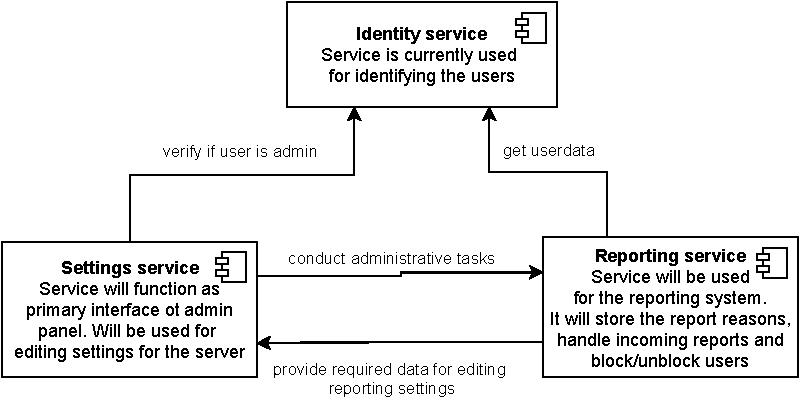
\includegraphics[width=1.0\textwidth]{./graphics/component_interaction}
    \caption{Service interaction concept designed for admin panel}
    \label{fig:componentInteraction}
\end{figure}

The \hyperref[subsubsec:settingsSer]{\textbf{settings service}} will function as the REST interface to the admin panel.
To this point it will interact with the identity service for verifying if the settings are actually being changed by an
administrator user.
It will also work with the \hyperref[subsubsec:reportingSer]{\textbf{reporting service}}: the service in charge of
handling the reporting system, to conduct administrative tasks like changing the reasons people can be reported for.

\begin{figure}[H]
    \centering
    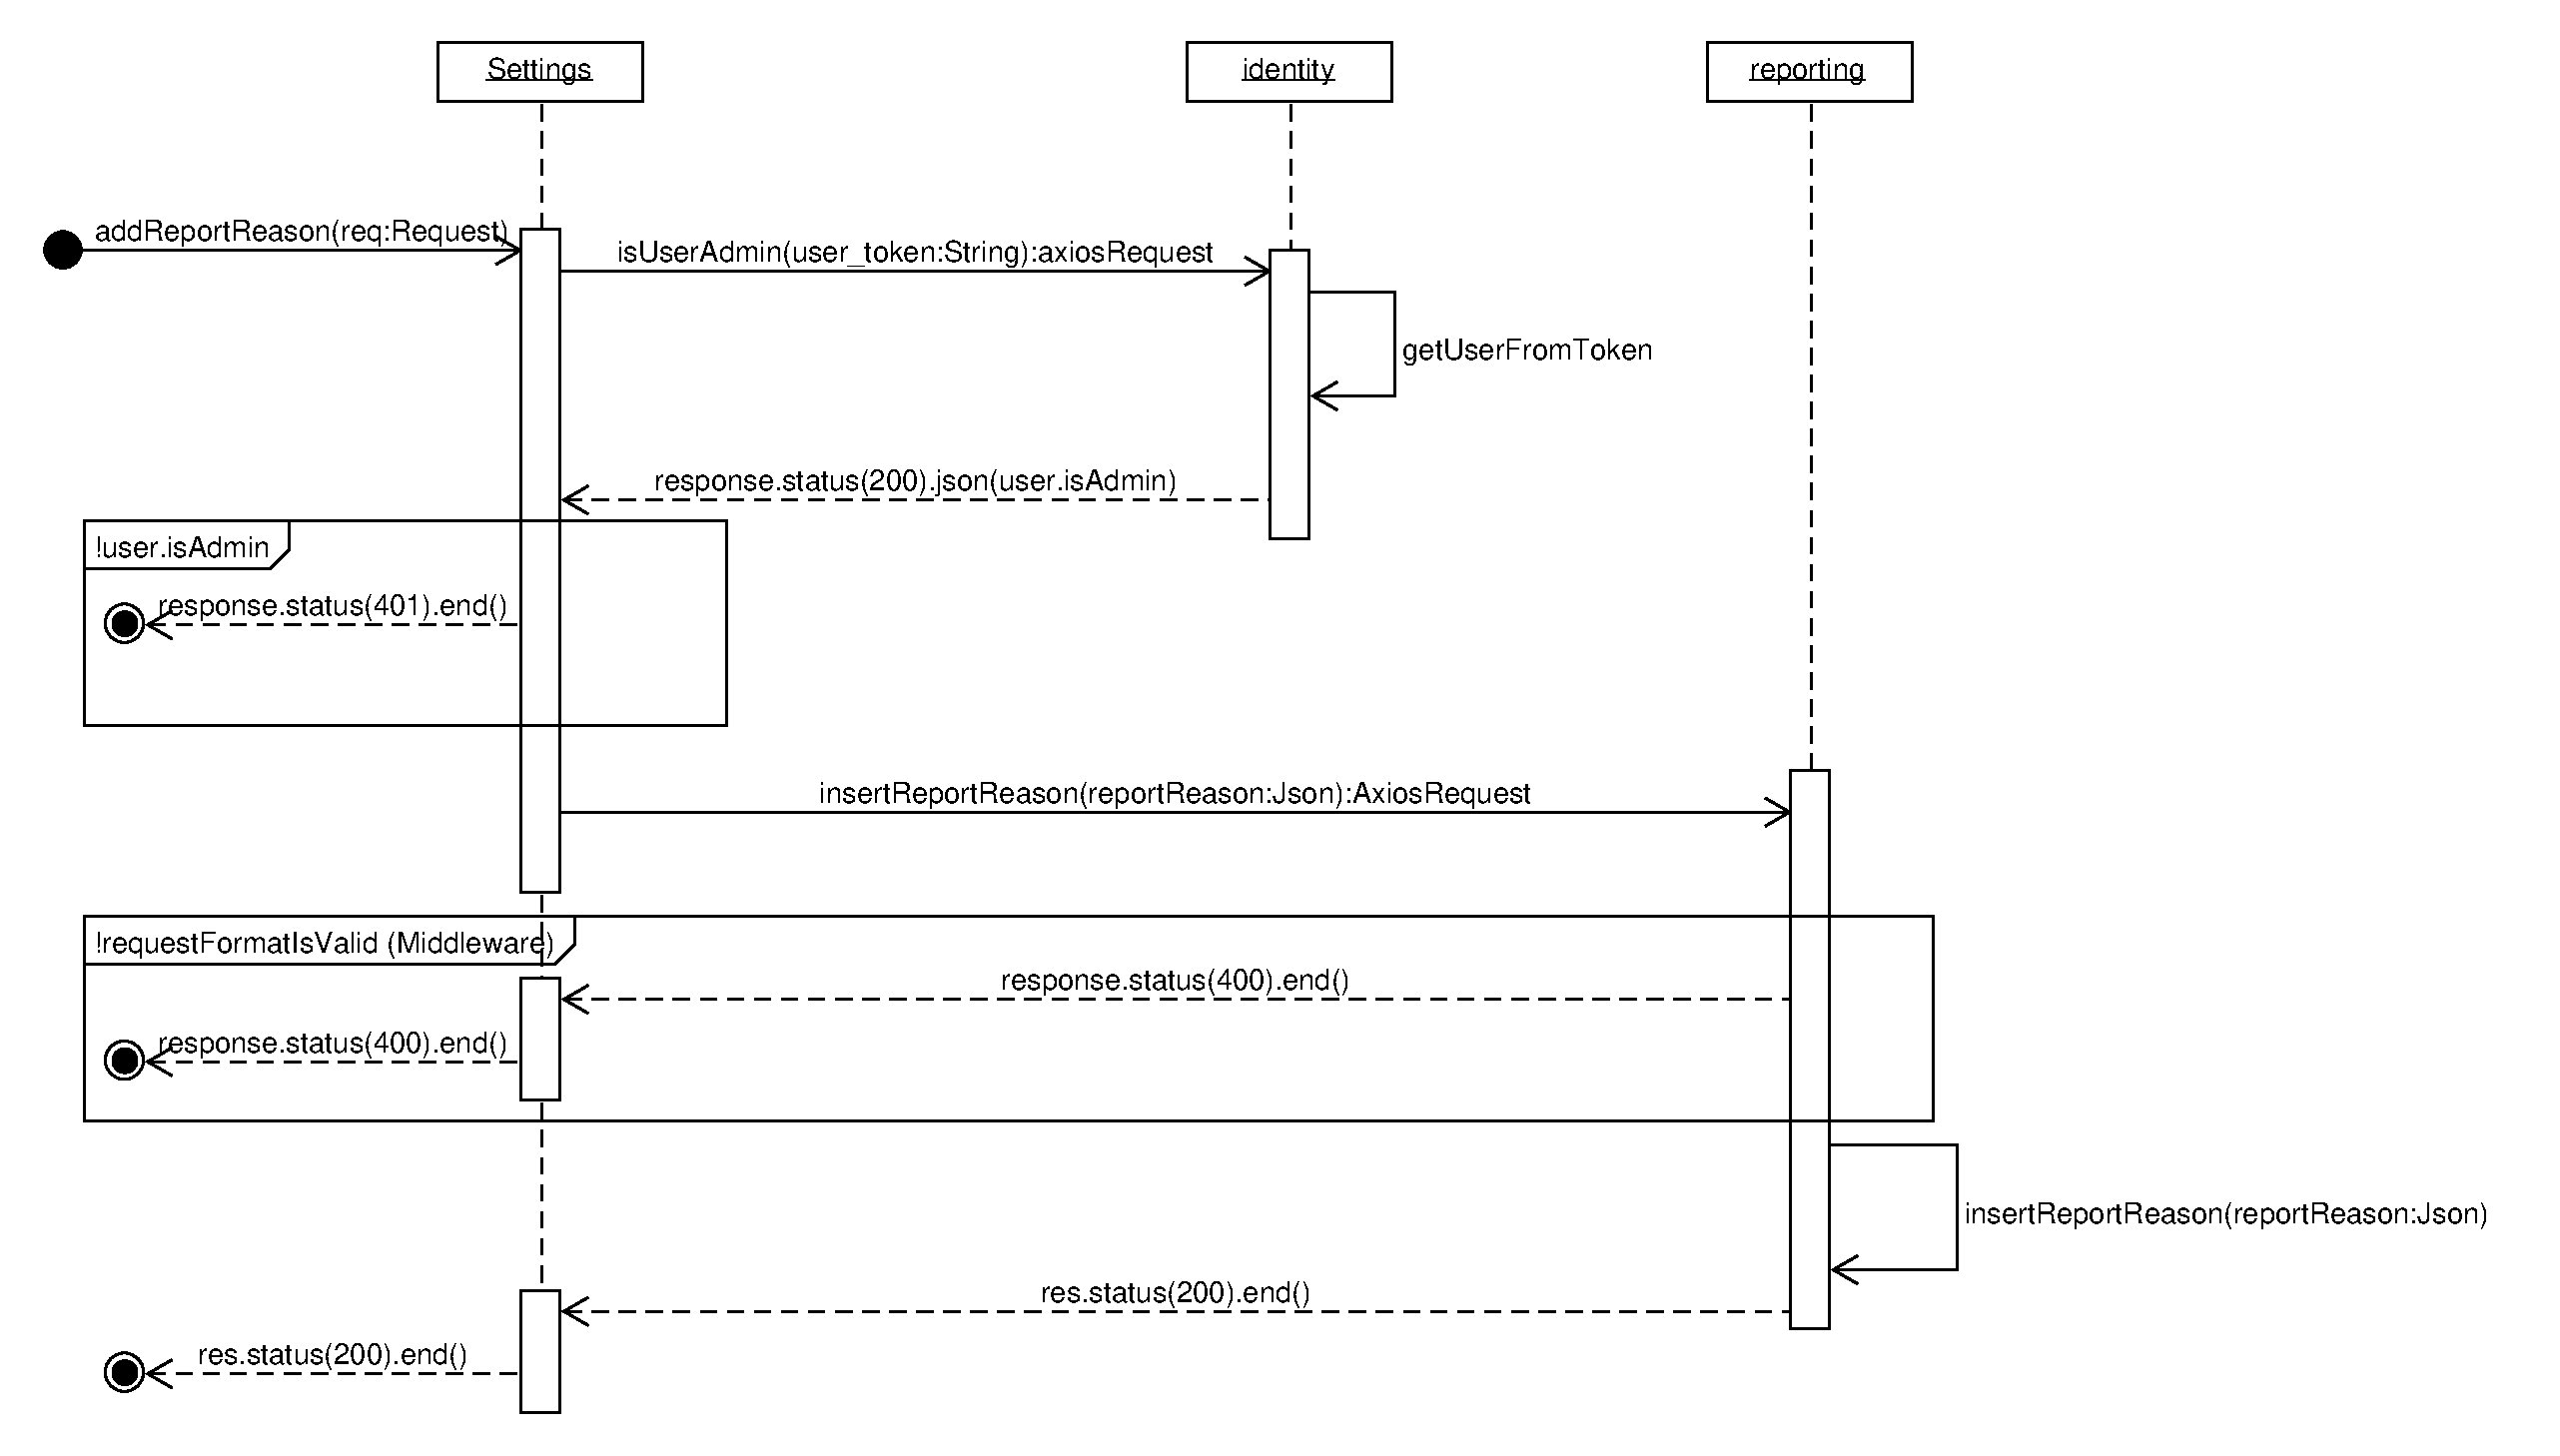
\includegraphics[width=1.0\textwidth]{./graphics/SequenceDiagram_AddReportReason}
    \caption{Service interaction concept designed for admin panel}
    \label{fig:sequenceDiagramAddReportReason}
\end{figure}

Figure~\ref{fig:sequenceDiagramAddReportReason} shows the sequence diagram for conducting the administrative task of
adding a report reason.
This diagram has been created in order to further visualize the responsibility and interaction between the existing
\hyperref[subsubsec:identitySer]{\textbf{identity service}}, and the two other services (settings and reporting).
Further information on this can be derived from~\hyperref[subsubsec:settingsSer]{\textbf{settings service}}.

\begin{figure}[H]
    \centering
    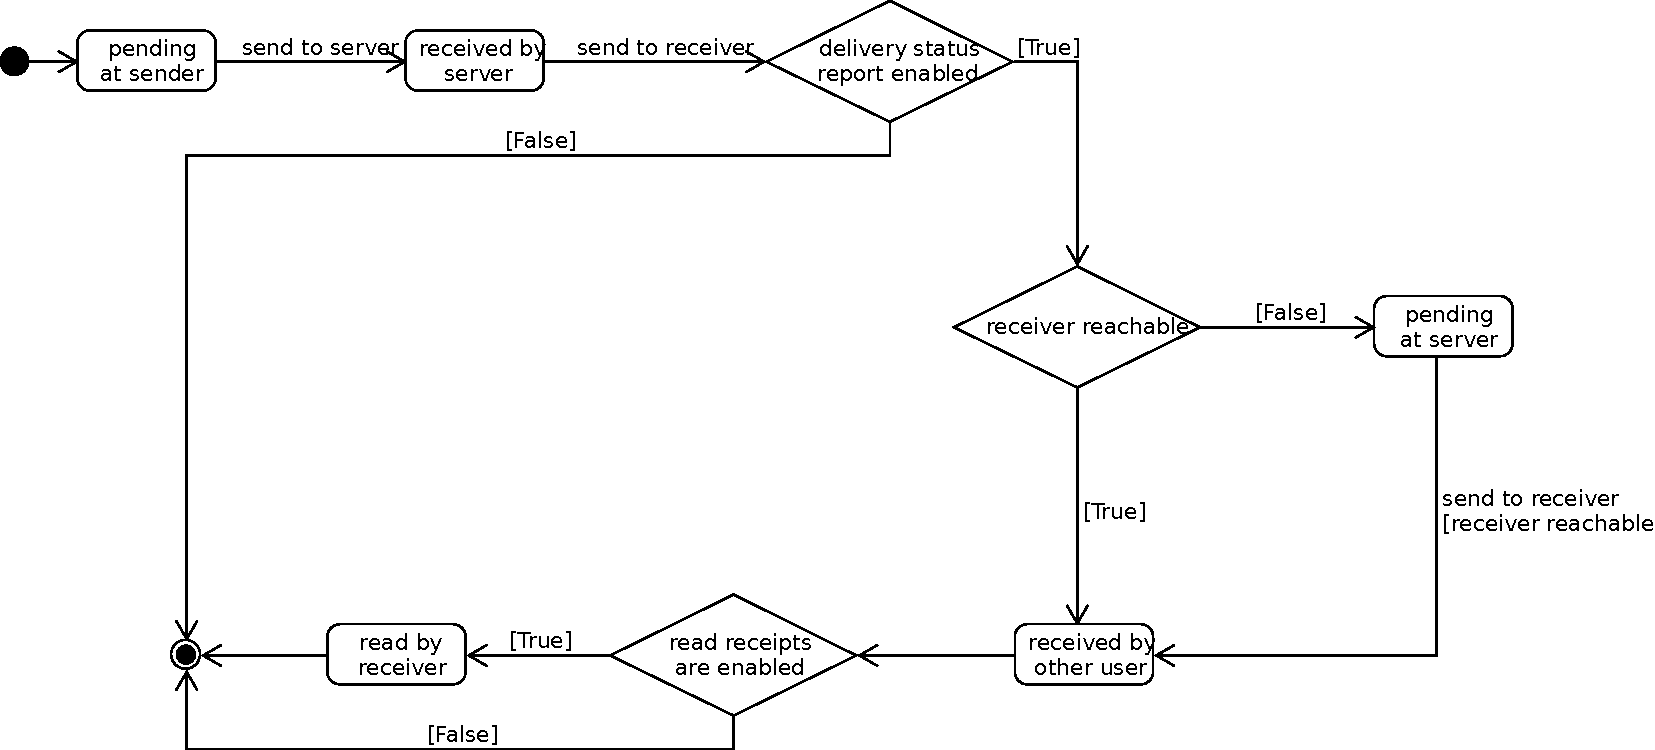
\includegraphics[width=1.0\textwidth]{./graphics/stateMachineMessage}
    \caption{State machine diagram for the message}
    \label{fig:stateMachineMessage}
\end{figure}

Figure~\ref{fig:stateMachineMessage} shows the different states of the message.
First the message will be in the \textit{pending at sender} stage, once the message has been successfully sent to the
server, it will enter the \textit{received by server} stage.
From there on it depends on the settings of the user, whether the delivers status report is enabled or not.
Should this option be disabled, the diagram ends here, otherwise, it will be checked if the receiver is reachable or
not.
If he is not reachable the state will be set to \textit{pending at server} until the message has been received by the
intended user, in which case the state will jump to \textit{received by other user}.
Should the other user be immediately reachable, the state of the message will directly change to the
\textit{received by other user state}.
Next, it again depends on the settings, whether read receipts are enabled or not.
If they are not enabled the diagram ends here, otherwise the message state will be set to \textit{read by receiver}
and the diagram ends here.

\begin{figure}[H]
    \centering
    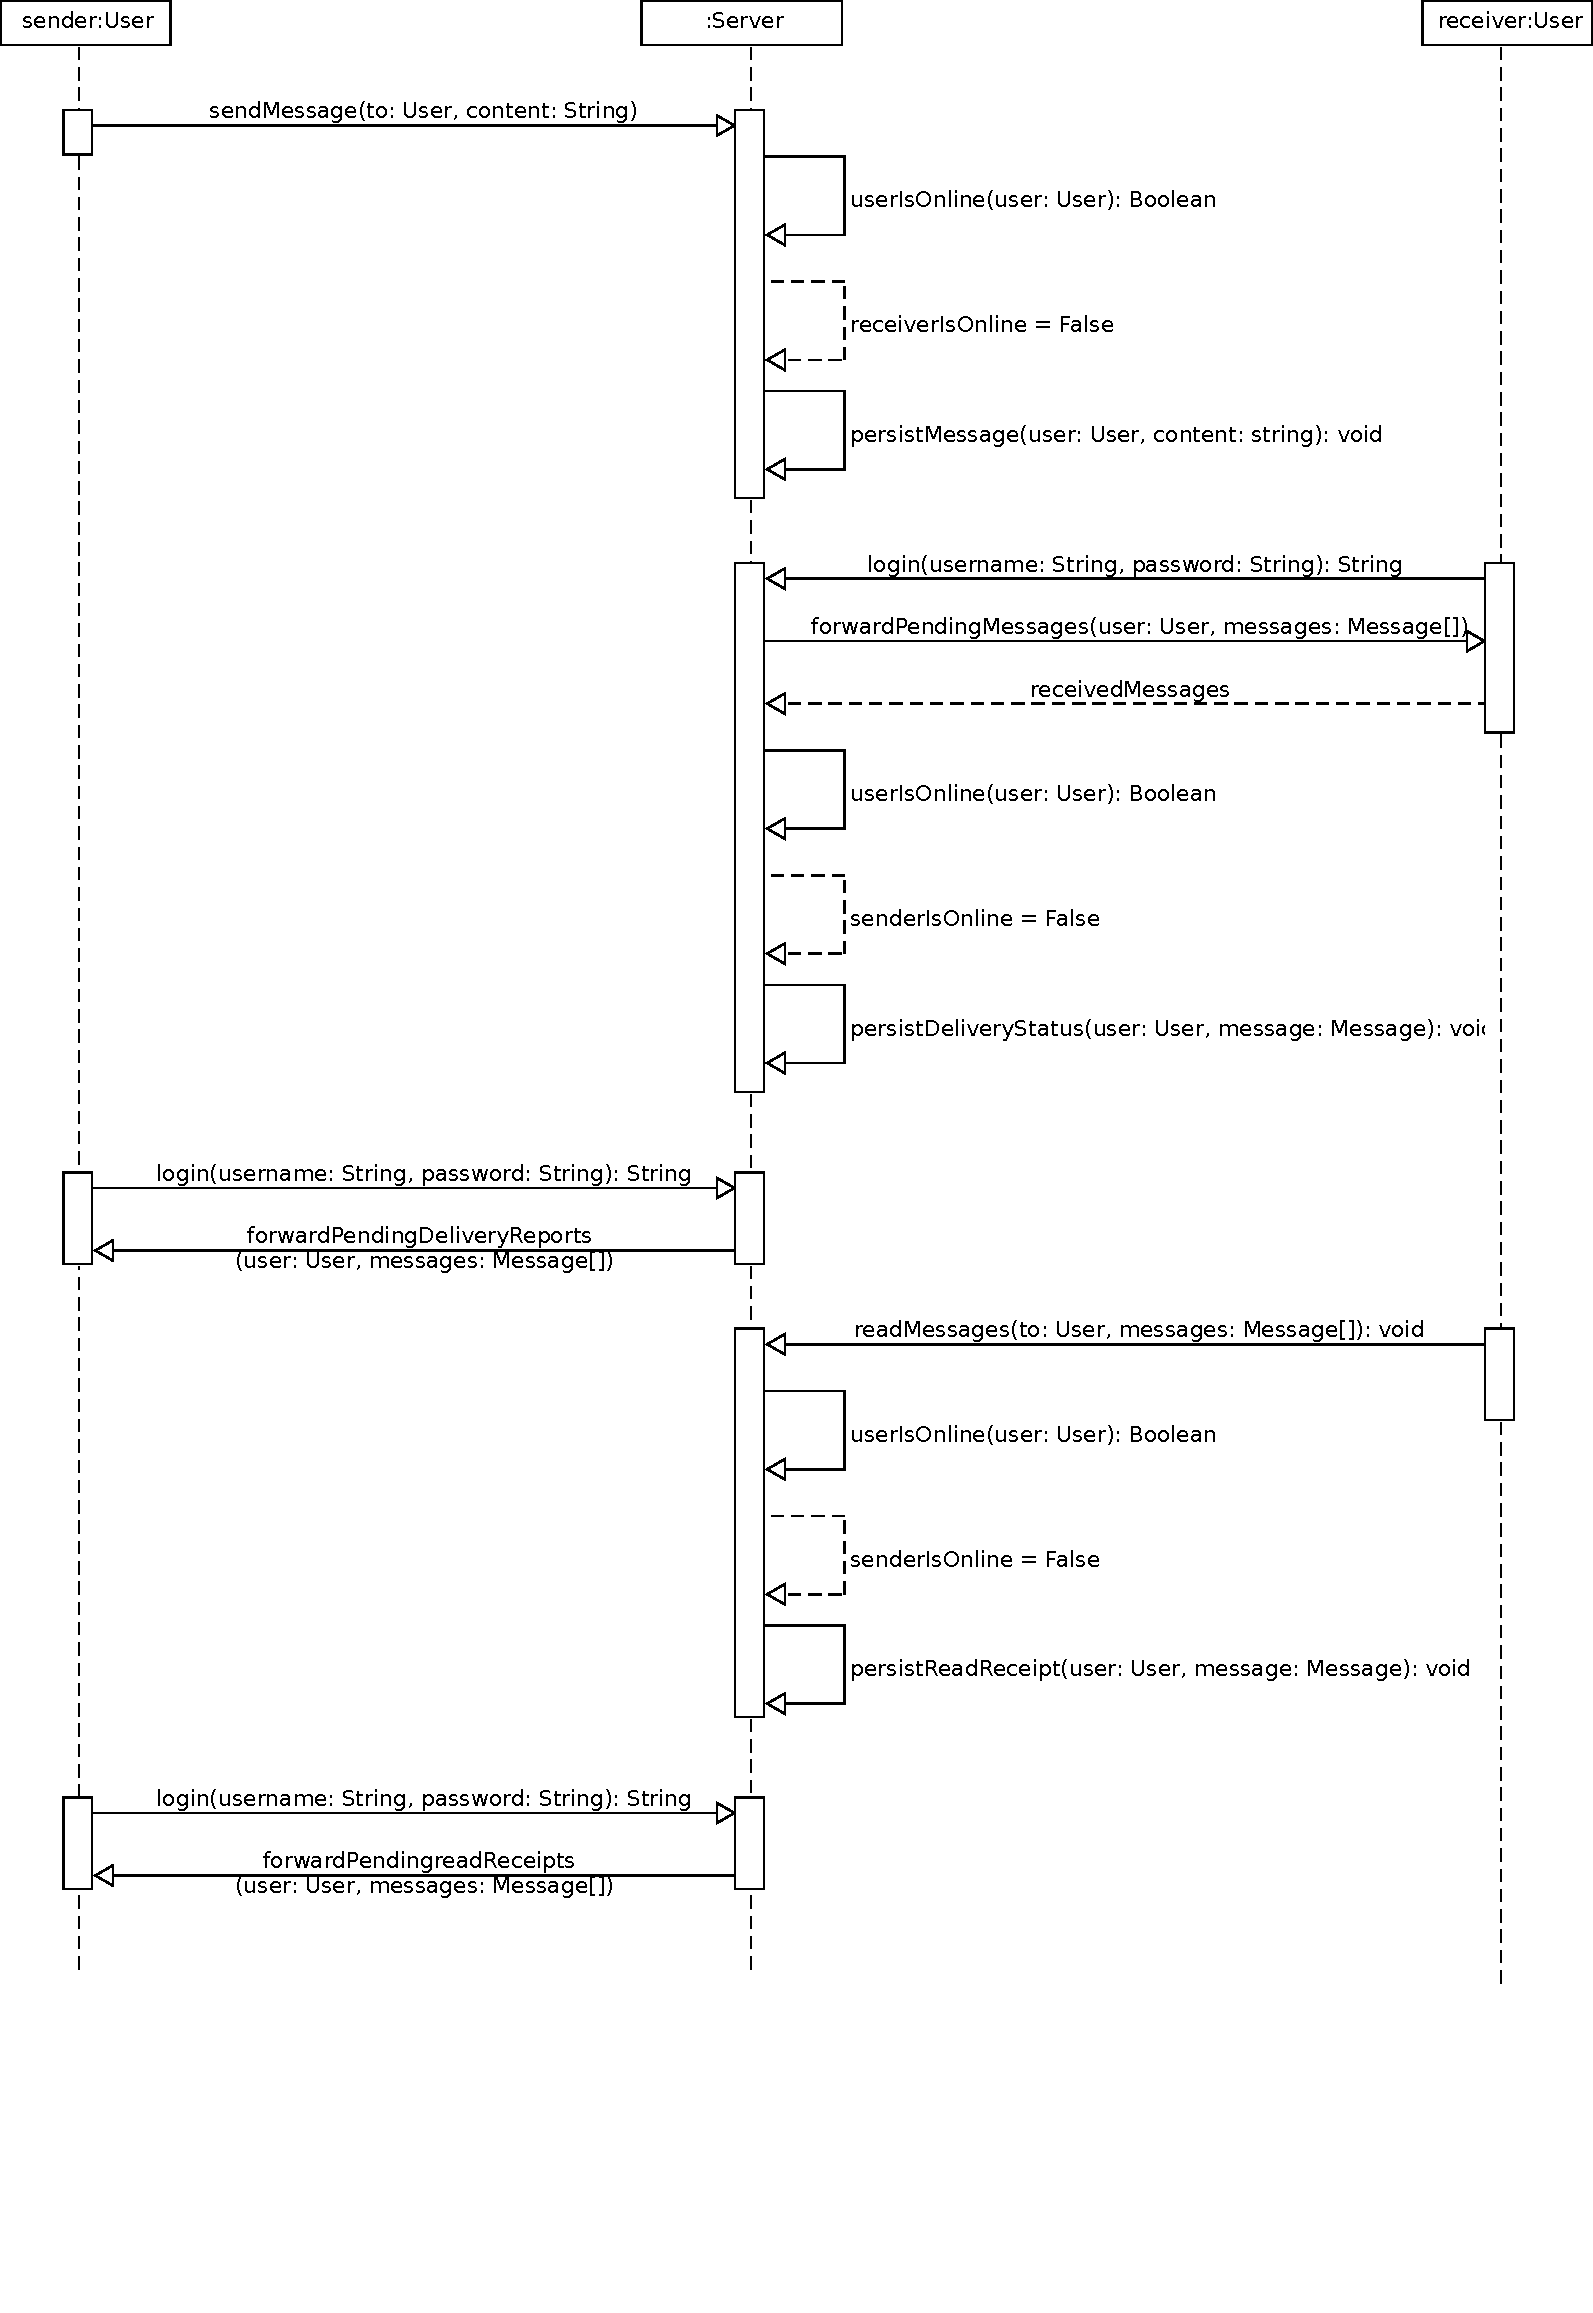
\includegraphics[width=1.0\textwidth]{./graphics/sequenceDiagramMessage}
    \caption{Sequence diagram for sending messages}
    \label{fig:sequenceDiagramMessage}
\end{figure}

Figure~\ref{fig:sequenceDiagramMessage} shows the sequence of sending a message.
This diagram will assume that all the worst cases (receiver is not online for receiving the message and sender is not
there for receiving status updates on the receipt and read receipt status of the message) in order to present how
forwarding of this information will be handled.
The sender sends the message to a certain recipient.
The server then checks if the receiver is online.
In this case he is not (receiverIsOnline = false).
The server will now temporarily store the message (persistMessage) until the recipient has logged in.
As soon as the recipient has logged in the server will forward the pending messages to the receiver.
The receiver client will then let the server know that the message has been received.
The server will now check if the sender is online to forward the delivery update.
In this case the sender is offline (senderIsOnline = false).
The server will now temporarily store the delivery update.
Once the sender has logged in, this will prompt the server to forward the delivery status to the sender.
The recipient at a later point in time will read the message and forward this a read status to the server.
The server will check if the sender is online which he in this case again is not.
Once the sender is logged in the sender will then forward the read receipt status.


\section{Network Design}\label{sec:network-design}

This section covers in detail how the actual software components are set up and how they are linked together.

\subsection{Application System Layers}\label{subsec:application-system-layers}

The following visualization (\ref{fig:figure33}) shows the interaction between the different components in the client
and server application.
It shows in detail how the different concrete parts depend on and communicate with each other.

\begin{figure}[H]
    \centering
    \caption{Trale System Layers and Deployment Diagram}
    \hspace*{-2.9cm}
    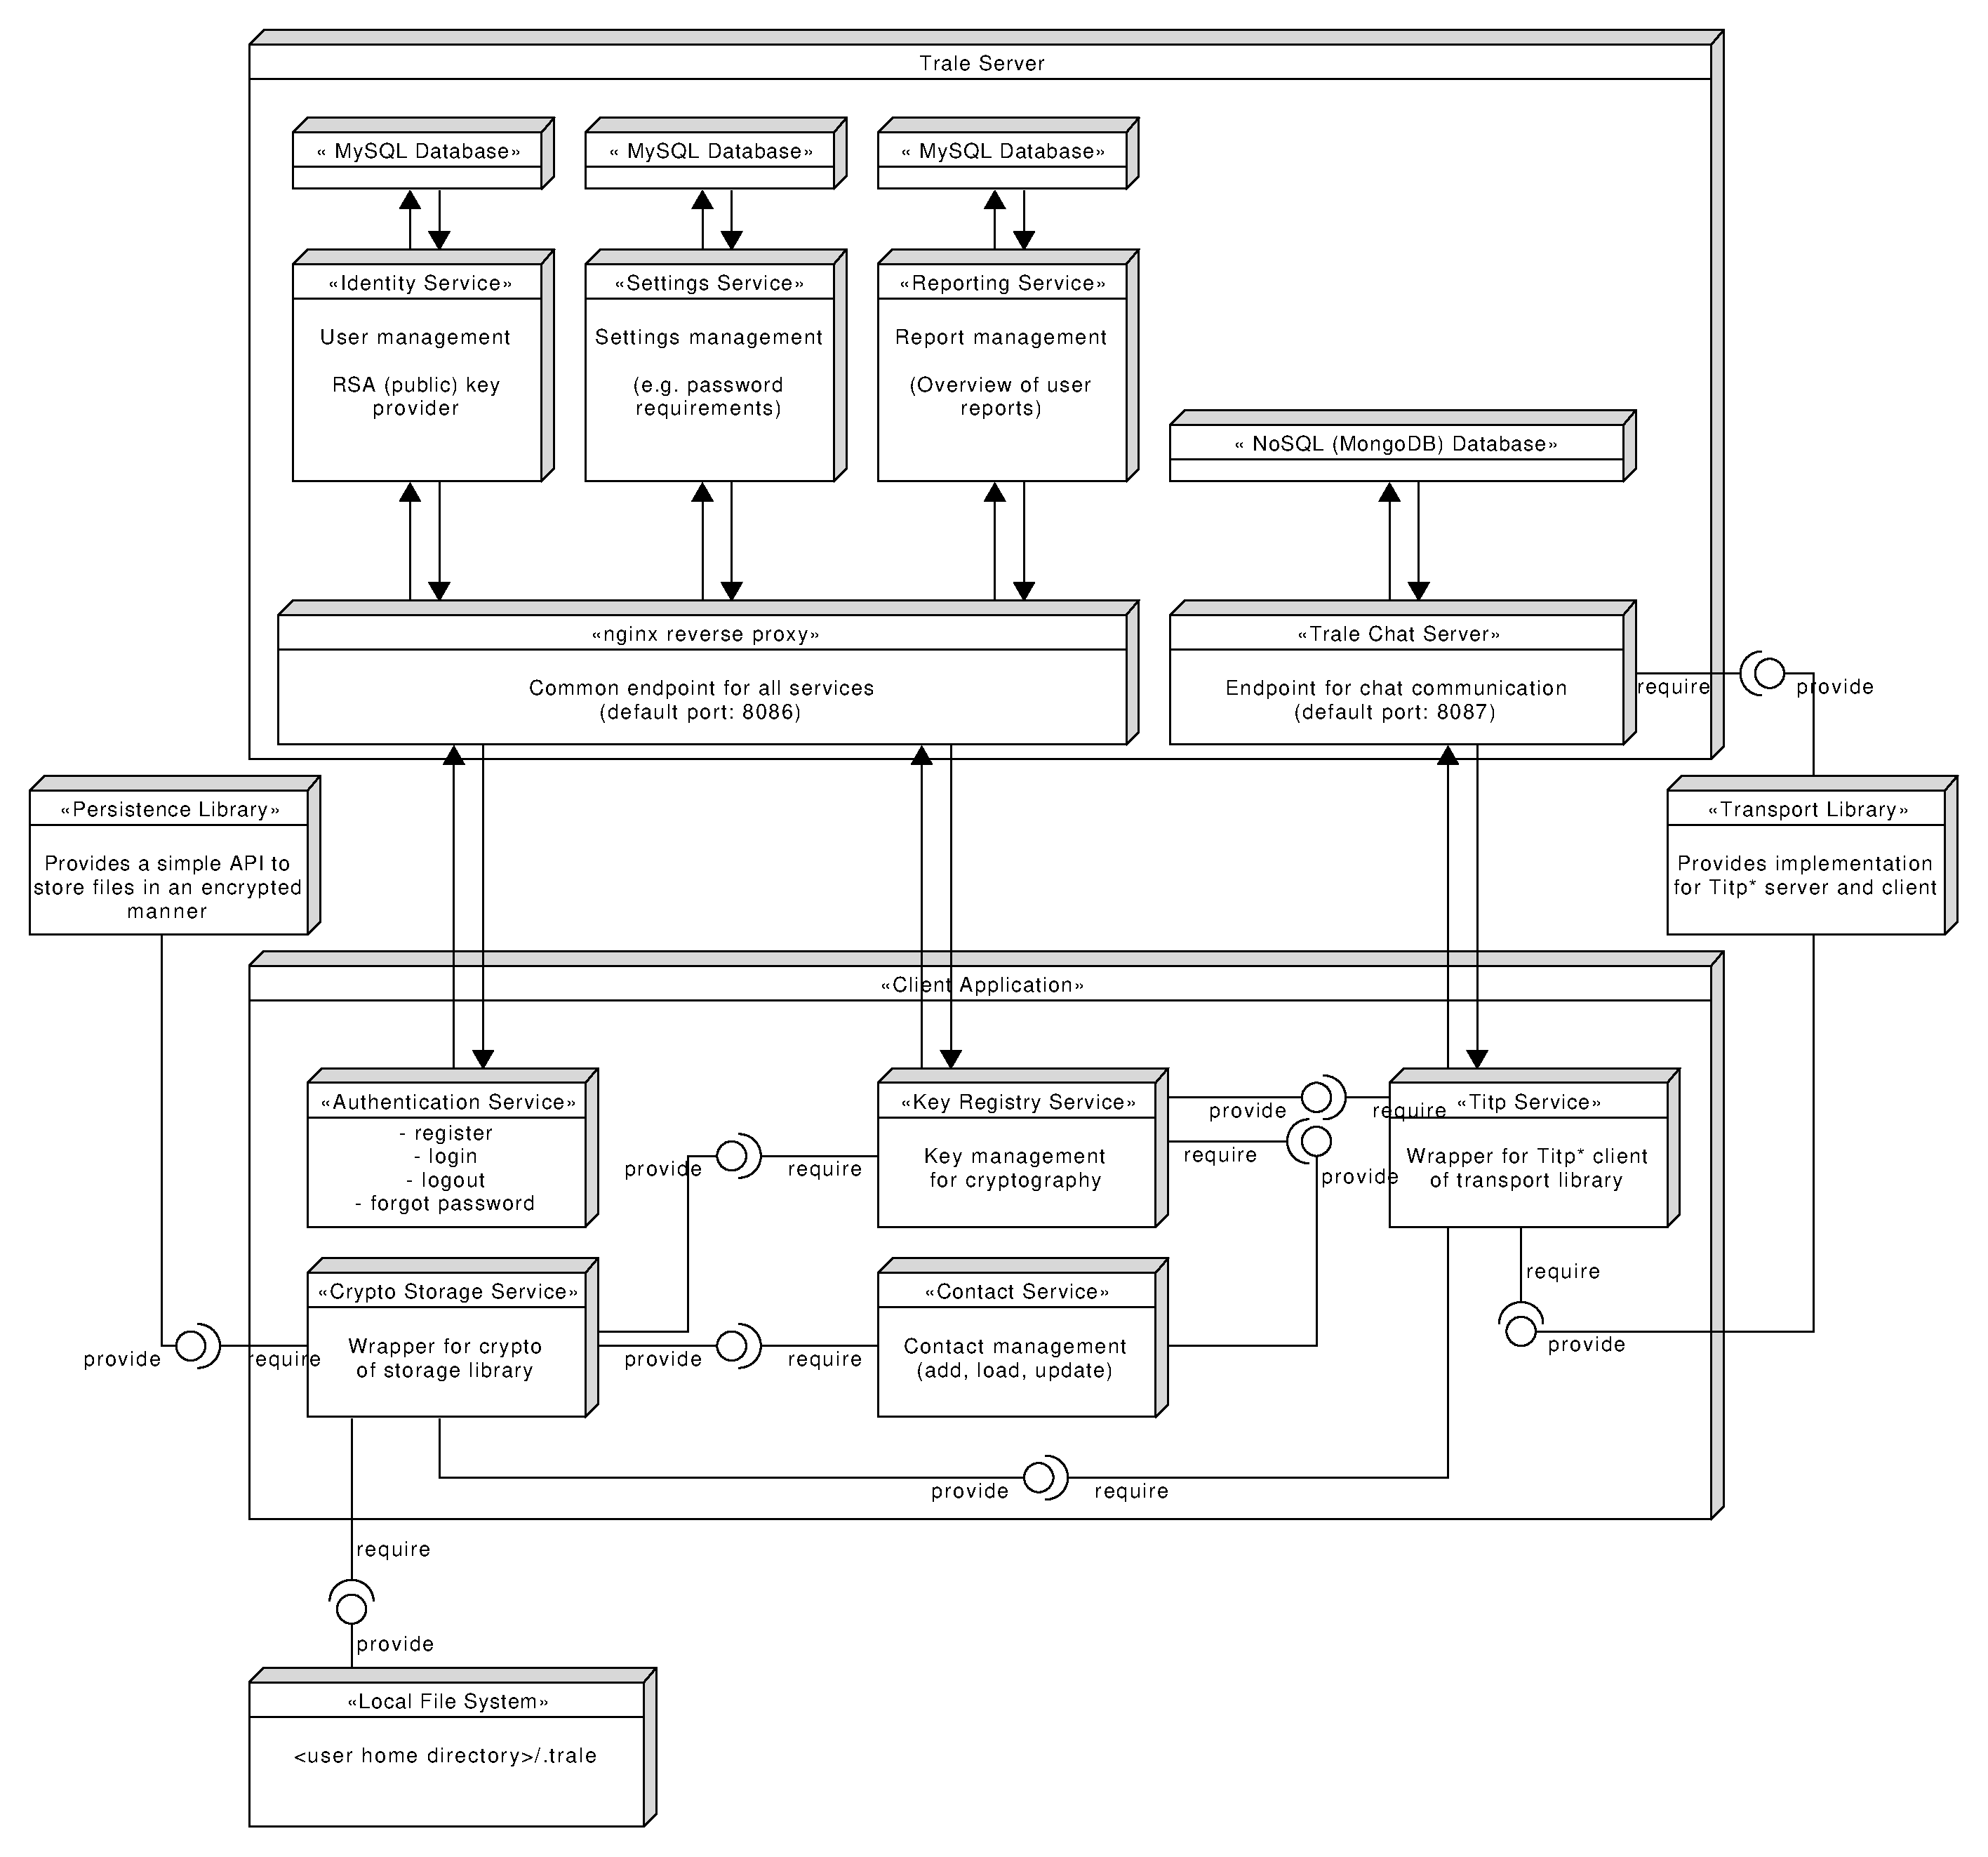
\includegraphics[width=1.3\textwidth]{./graphics/systemLayers}
    \label{fig:figure33}
\end{figure}
\textit{*Titp} stands for \ac{titp}, which will be covered in the section
\hyperref[subsec:transport]{\textbf{transport library}}.

\subsection{Network Architecture}\label{subsec:network-architecture}

The previous diagram (\ref{fig:figure33}) showed how the system is build up in general.
The following diagram shows how participants on many systems may communicate with one-another.

In the example below (\ref{fig:figure32}), Alice and Bob are connected to the same server (A).
They can communicate with each other.
However, they can also communicate with Charly who is located on a different server (B).
The servers are communicating with each other on the users behalf and forward the messages without fully knowing
the conversation partners.
With this approach the sender stays pseudo-anonymous to the receiver and the receiver's server and the opposite way
around.

\begin{figure}[H]
    \centering
    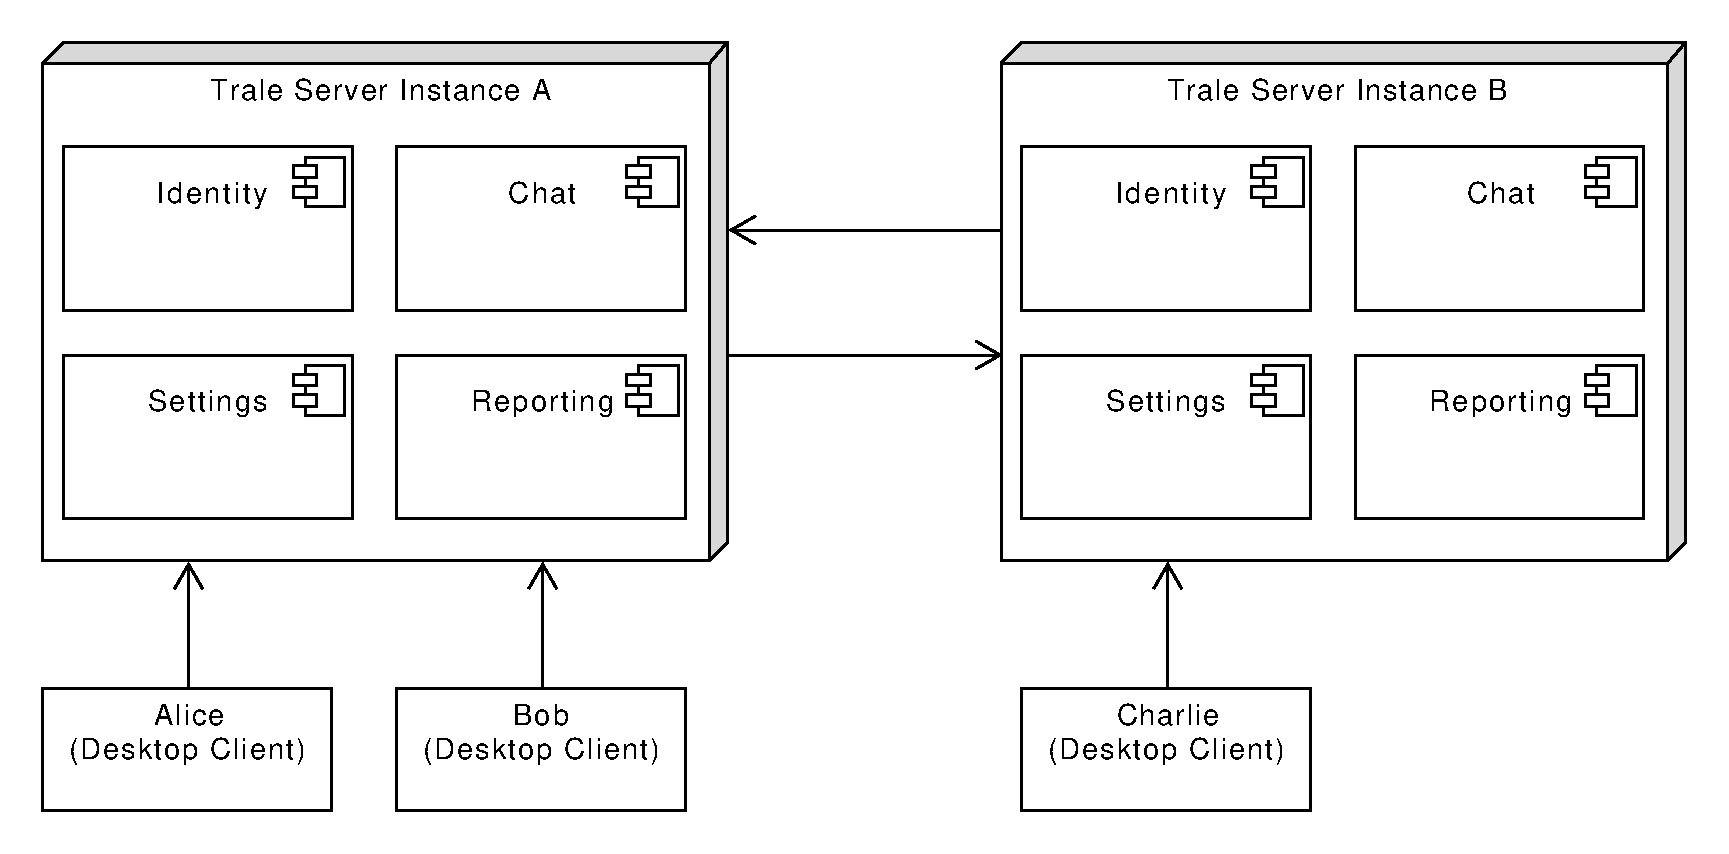
\includegraphics[width=1.0\textwidth]{./graphics/components}
    \caption{Trale Network Architecture}
    \label{fig:figure32}
\end{figure}

\subsection{Port distribution}\label{subsec:port-distribution}

The following table shows all utilized ports of the server side.
External ports are reachable from client applications.
The internal ports are used for inter-service communication.

\begin{table}[H]
    \centering
    \begin{tabular}{|l|l|l|}
        \toprule
        \textbf{Port} & \textbf{Port Type} & \textbf{Service}                               \\
        \midrule
        8086          & External & Default \ac{http} Port (see~\ref{fig:figure33})     \\
        \midrule
        8087          & External & Default \ac{titp} Port (see~\ref{fig:figure33})     \\
        \midrule
        3000          & Internal & Identity Service                               \\
        \midrule
        3001          & Internal & Chat service over \ac{http}                         \\
        \midrule
        3002          & Internal & Chat service over Trale connection \\
        \bottomrule
    \end{tabular}\label{tab:table}
\end{table}

